\documentclass{article}
\usepackage{graphicx}
\usepackage{caption}
\usepackage{svg}
\usepackage{subcaption}
\usepackage{hyperref}
\usepackage{cleveref}
\usepackage{adjustbox}
\usepackage{listings}

\graphicspath{{./images/}}

\hypersetup{
    colorlinks=true,
    linkcolor=blue,
    filecolor=magenta,      
    urlcolor=cyan,
    pdftitle={Presentation},
    pdfpagemode=FullScreen,
}

\title{h550 project - Security assessment of an AP}
\author{Esteban Aguililla Klein}
\begin{document}
\maketitle	
\tableofcontents
\newpage
\section{Introduction}
Nowadays most IOT devices contain some flavor of a vulnerability, backdoor or critical bug. However, those problems in some cases are never fixed as IoT devices are dependent on their vendors for firmware update due their code being proprietary (in most cases). Furthermore, some users might forget (or not know) that their device's software is not updated and by extension, vulnerable. The goal of this project is to show how easy or un-easy it is to dump, find and exploit an access point.
\subsection{Context}
In this section we will explain what the target is and what are the settings and boundaries of the analysis.
\subsection{Device}
The device is an access point from Cisco released in October 2008, aimed at small businesses. This products has been discontinued in 2019 and its sales ended back in 2014.
\begin{figure}[!h]
	\centering
	\begin{subfigure}{0.3\textwidth}
		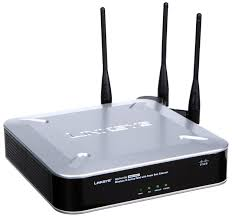
\includegraphics[width=\textwidth]{AP.jpg}
		\caption{Product picture}
		\label{outside}
	\end{subfigure}
	\begin{subfigure}{0.3\textwidth}
		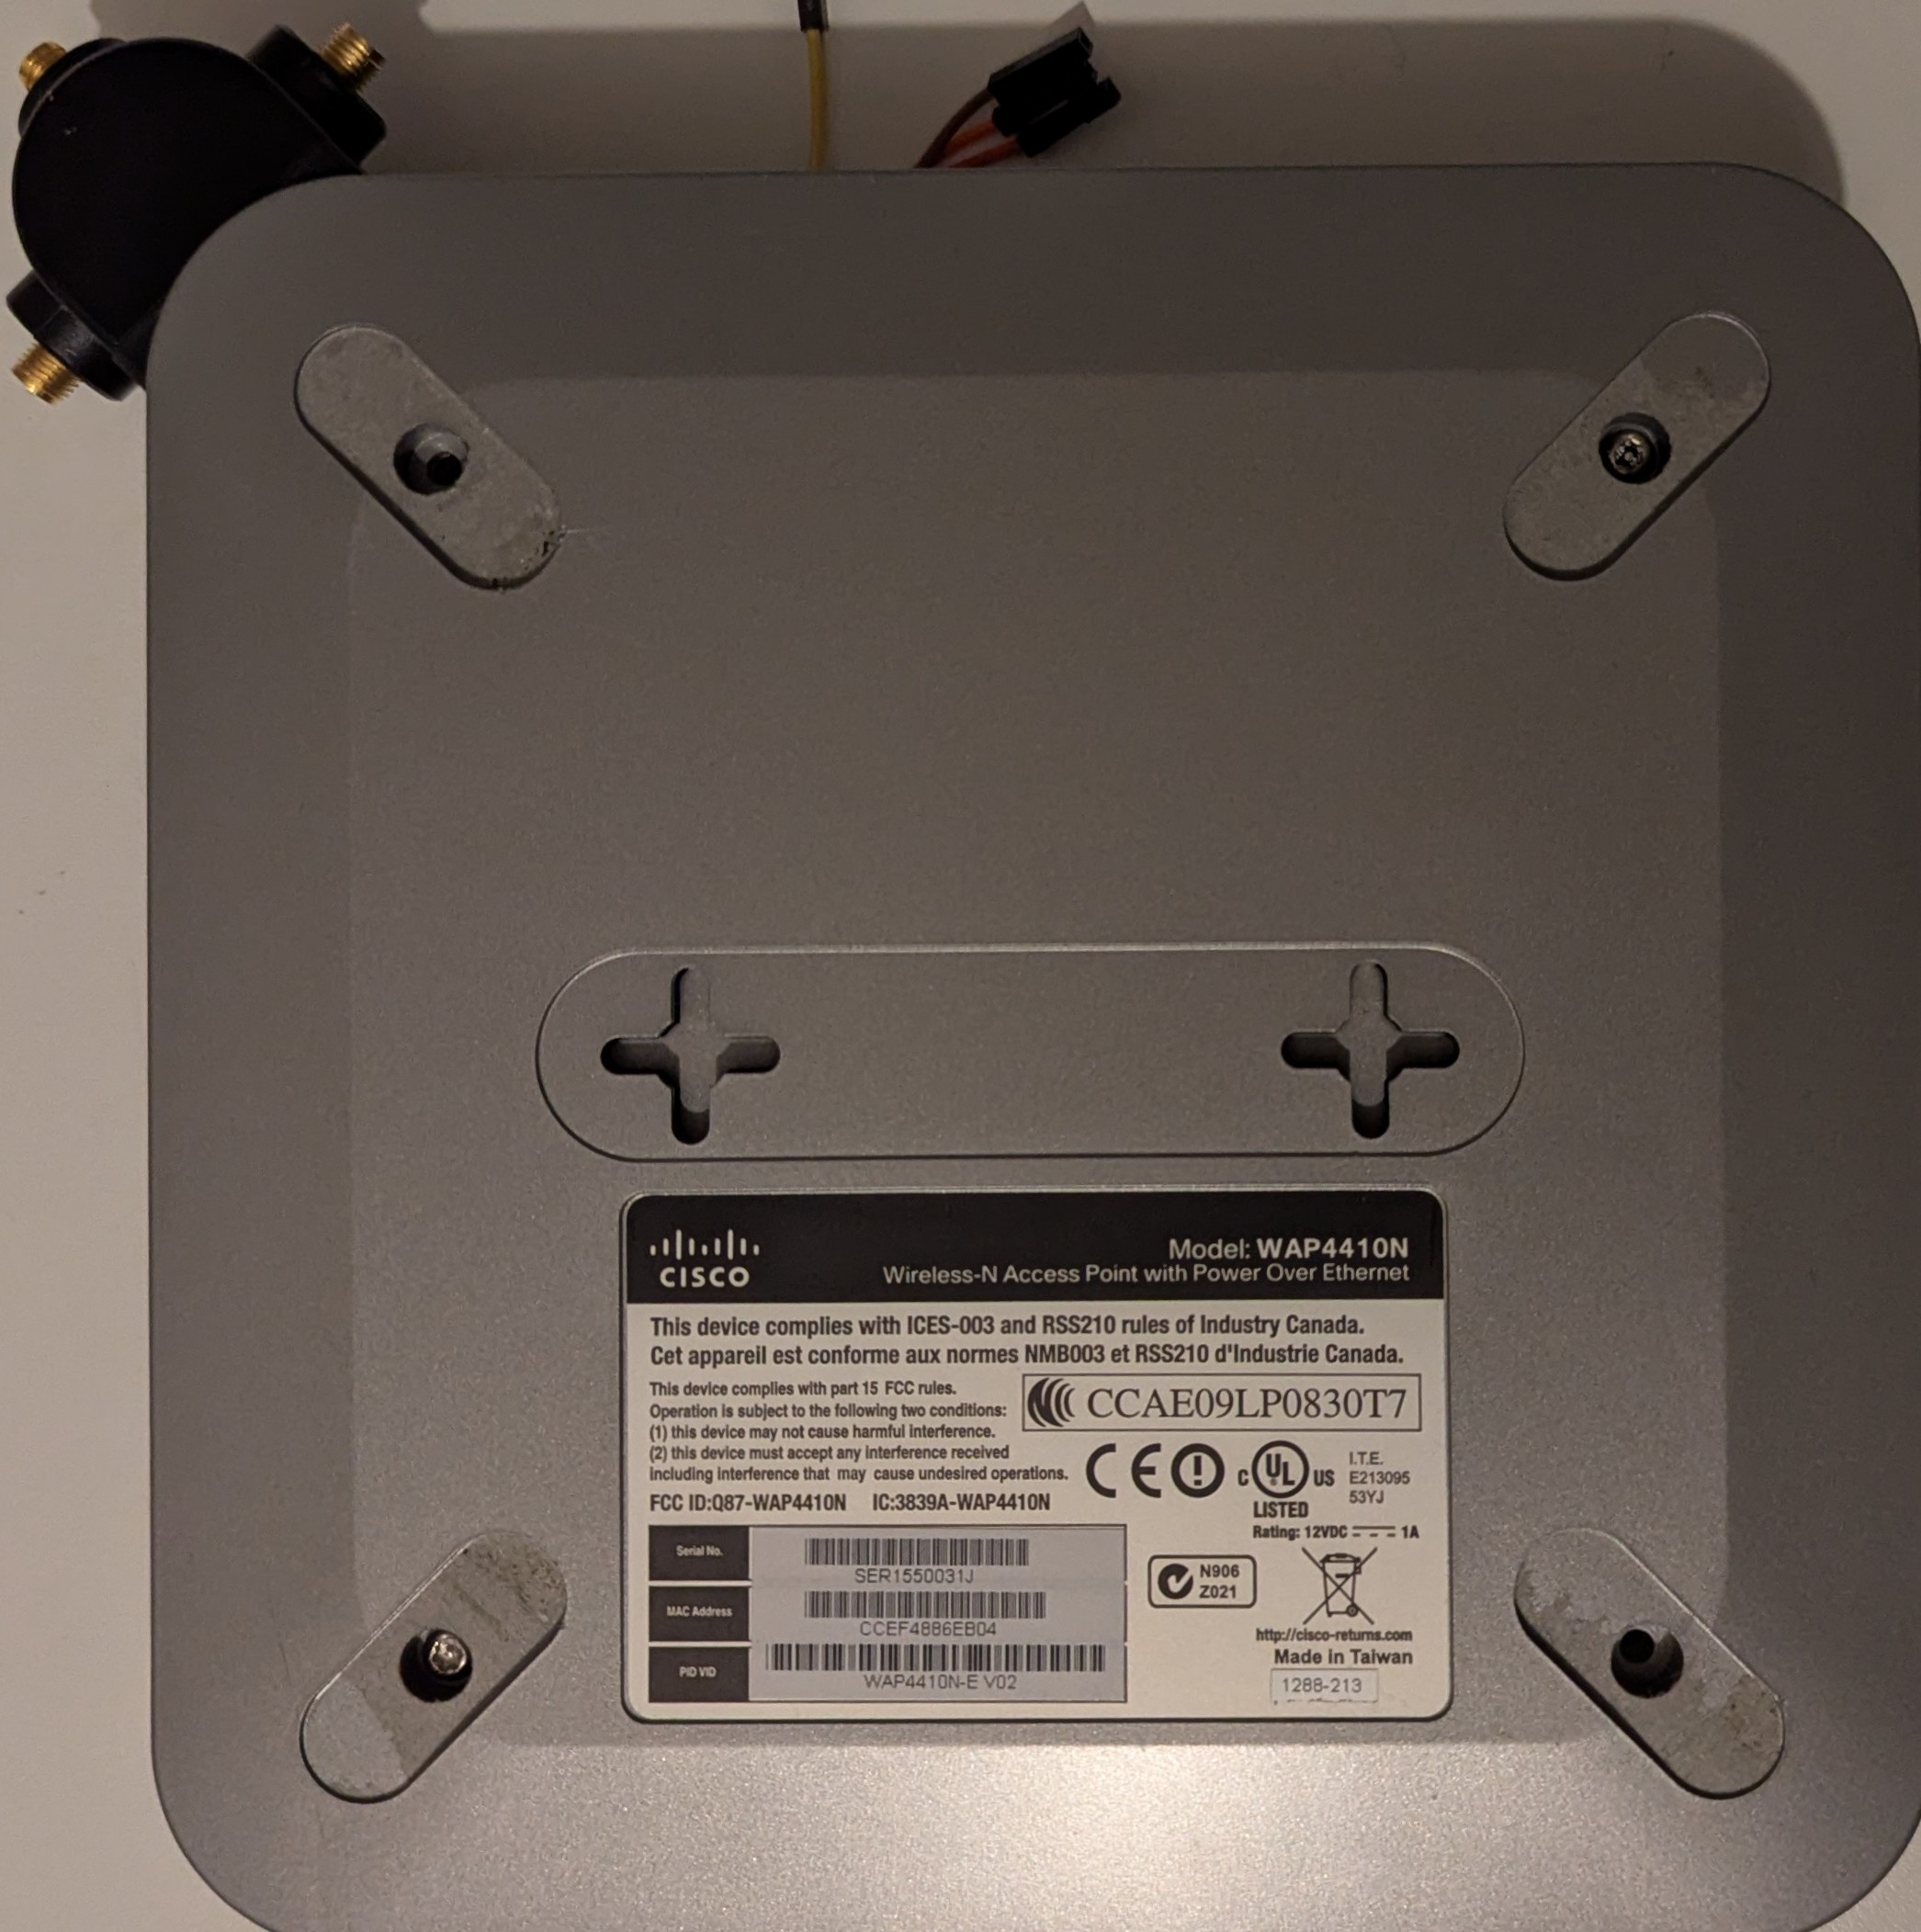
\includegraphics[width=\textwidth]{bottom.jpg}
		\caption{Bottom}
		\label{bottom}
	\end{subfigure}
	\begin{subfigure}{0.3\textwidth}
		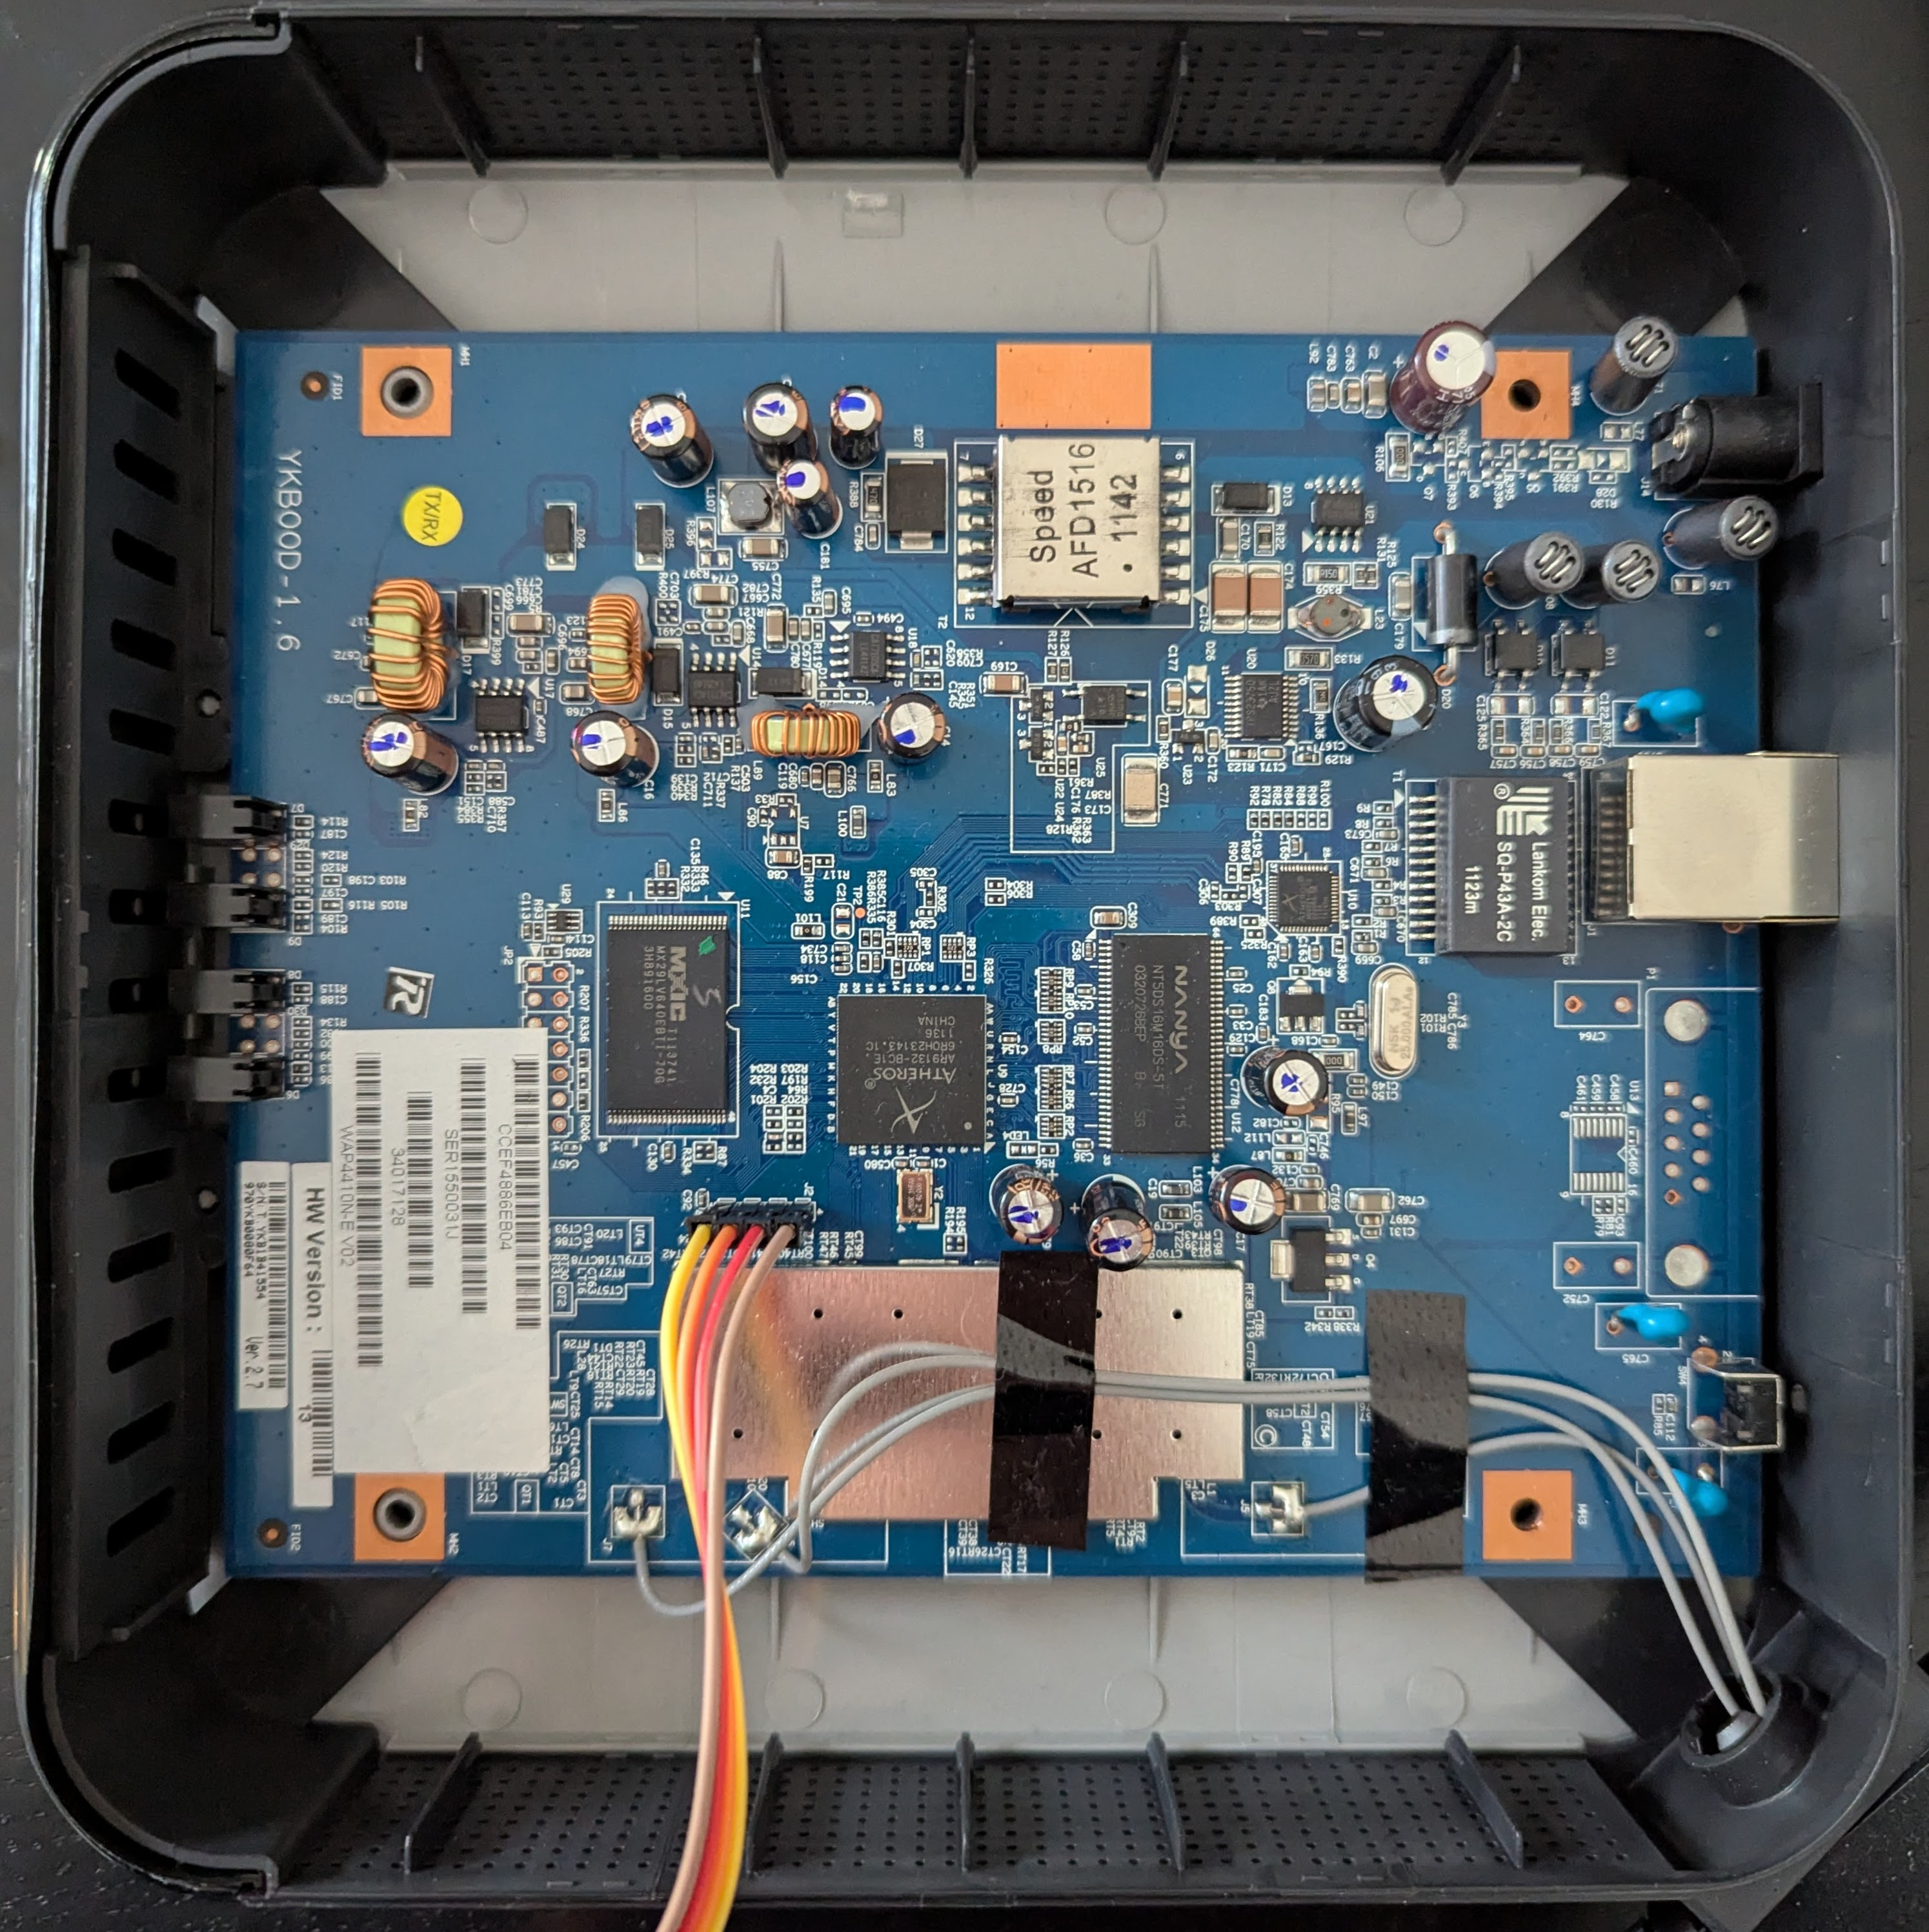
\includegraphics[width=\textwidth]{inside.jpg}
		\caption{Inside}
		\label{inside}
	\end{subfigure}
	\caption{Pictures of of the WAP4410N}
	\label{wap4410n}
\end{figure}

The device can be powered up using a barrel adapter or through PoE which hints at its purpose being ease of batch deployment. On the network side, it support 802.11n, 802.11g and 802.11b. With the time period in mind, and, for 802.11b and g, the only supported encryption protocol was WEP (64/128 bits in this case). Also, firmware updates were handled through the web portal (as there is no I/O) sadly, they are down. On figure \ref{inside}, we can see a cable going outside of the device, this is the UART access which was enabled by default. Most of the remaining ICs are irrelevant/too old to be told apart because of wear of the imprint and/or arcane references.
\subsection{Lab setup}
The testing setup is made of the WAP4410N, a router and my computer : for simplicity sake, the router is out of scope from this analysis and all its security features are disabled. The computer has a  wireless connection to the AP.
\begin{figure}[!ht]
	\includesvg[width=\textwidth]{images/lab.svg}	
	\caption{Lab setup}
\end{figure}

\noindent The equipment that I used was very minimal,

\begin{figure}[!ht]
\begin{tabular}{|c|c|}
	\hline
	hardware & software \\
	\hline
	Wireshark & FT232 board USB-A UART adapter \\
	GNU Screen, xxd, dd, binwalk, squashfs-utils, nmap & Multimeter \\
	radare2, ghidra & Dupont Cables\\
	\hline
\end{tabular}
\caption{List of used software/hardware}
\end{figure}


At first, I intended to use a SPI programmer (CH341a) to dump the firmware more easily using \href{https://github.com/flashrom/flashrom}{flashrom}. However, as we will see in later section it was not feasible in this context without specialized hardware toosl. On the software side, there are no real limitations as most of the state of the art tools are free and open source (with the exception of IDA).
\section{Reconnaissance}
In this section, we will discuss the reconnaissance of our device. This part was inspired by the first step in the cyber kill chain (which will be vaguely followed throughout the following sections). We will proceed in a bottom up approach in regards to the level of abstraction : from hardware to software
\newpage
\subsection{Physical}
\paragraph{Teardown} The device is held together by four 8-points screws under rubber feets which indicates that it wasn't meant to be opened (nor repaired \dots). Once inside, most of the device is empty and everything is available without further need to dismantle it. 

\paragraph{IC reconnaissance} At this point we can start looking for interesting ICs like flash memory or processors :

\\
\begin{minipage}[t]{0.3\textwidth}
	\adjustimage{angle=90, valign=t}{images/flash.png}
\end{minipage} %
\vspace{0.5cm}
\hfill
\begin{minipage}[t]{0.7\textwidth}
	\begin{itemize}
		\itemsep0em
		\item reference : \href{https://www.alldatasheet.com/datasheet-pdf/view/267962/MCNIX/MX29LV640DBTC-90G.html}{MX29LV640DBTC-90G}
		\item format : 48 TSOP
		\item manufacturer : Macronix
		\item size : ~8MB
	\end{itemize}
\end{minipage}
\begin{minipage}[t]{0.3\textwidth}
	\adjustimage{width=\textwidth, angle=180, valign=t}{images/cpu.png}
\end{minipage} %
\vspace{0.5cm}
\hfill
\begin{minipage}[t]{0.7\textwidth}
	\begin{itemize}
		\item family : Atheros 9100
		\item reference : Atheros9132
		\item manufacturer : Qualcomm
		\item architecture : MIPS 24K V7.4 32bits
		\item endianness : big endian
		\item bogomips : 265.21
	\end{itemize}
\end{minipage}
\noindent The MIPS architecture is very common on embedded devices and very easy to reverse engineer its assembly. Regarding the NAND flash, it would as hinted before, it would require to de-solder the IC using a special SPI programmer (or an adapter for the ch341a).
\paragraph{Finding the UART} There are 4 header pin on the board, we will try them using a multimeter : the UART has a very specific behavior.

\begin{figure}[!ht]
	\includesvg[width=\textwidth]{images/uart.svg}
	\caption{UART connected through Dupont cables with labeled ports}
\end{figure}

\noindent Before taking measures, we must find the ground, to do so, can check continuity between a metal part (which should be grounded) and the ground pin from a known IC (in this case the flash). After making sure that a metal part is grounded we can start taking measurements,
\begin{figure}[!ht]
	\centering
	\begin{tabular}{|c|c|c|c|}
		\hline
		pin & $R_{VSS}$ & $V$ & info \\ 
		\hline
		1 & $8.6k\Omega$ & $\approx 3.3V$ & VCC \\
		2 & $\infty k\Omega$ & $\approx 0V - VCC$ & TX\\
		3 & $\infty k\Omega$ & $\approx 0V$ & RX \\
		4 & $0$ k $\Omega$ & $0V$ & GND \\
		\hline
	\end{tabular}
	\caption{Multimeter measurements}
\end{figure}

\noindent The voltage goes from 0V to the VCC, at startup because of the boot log outputs a lot of data. The Rx has a voltage of 0 as its used to receive data and doesn't send any. The next step is to try connecting the UART to the computer using a FT232, 
\begin{figure}[!ht]
	\centering
	\includesvg[width=\textwidth]{images/ft232.svg}
	\caption{UART to USB-A }
\end{figure}

\noident Regarding the baudrate, we can try 115200 as its the most common,
\begin{verbatim}
	screen /dev/ttyUSB0 115200
\end{verbatim} 
\subsection{Bootloader}
\begin{figure}[!ht]
\begin{verbatim}
ar7100> bdinfo
boot_params = 0x81F63FB0
memstart    = 0x80000000
memsize     = 0x02000000
flashstart  = 0xBF000000
flashsize   = 0x00800000
flashoffset = 0x0002F690
ethaddr     = CC:EF:48:86:EB:04
ip_addr     = 192.168.1.10
baudrate    = 115200 bps	
\end{verbatim}
\end{figure}
From the boot log we can get that the bootloader is U-Boot 1.1.4 which is a very common bootloader and open source solution. We can interrupt the autoboot and access the U-Boot console which is un-protected. The version of U-Boot is reduced, and there are "custom" commands for testing device specific features. We can dump some information about the device using some builtin commands. We learn that the devices uses a squashfs3 file system. 
\subsection{Console}
If we leave the autoboot alone, we get into a root Linux ash shell. There are device specific CLI commands and a reduced busybox. There is a fwversion command which tell us that the firmware version is 2.0.4.2. As we are already root, we can't really do any privilege escalation. Furthermore, as the device only has a squashfs3 file system we can't get any persistency.

\begin{verbatim}
Starting kernel ...

Linux version 2.6.15--LSDK-7.3.0.435 (root@apbs) 
	(gcc version 3.4.4) #36 Fri May 13 18:51:36 CST 2011

flash_size passed from bootloader = 8
arg 1: console=ttyS0,115200
arg 2: root=31:02
arg 3: rootfstype=jffs2
arg 4: init=/sbin/init
arg 5: mtdparts=ar9100-nor0:256k(u-boot),
	64k(u-boot-env),
	6464k(rootfs),
	1280k(uImage),
	64k(nvram),
	64k(calibration)
arg 6: mem=32M
...
Kernel command line: console=ttyS0,
	115200 root=31:02 rootfstype=squashfs init=/sbin/init mtdparts=ar9100-nor0:256k(u-boot),
	64k(u-boot-env),
	6464k(rootfs),
	1280k(uImage),
	64k(nvram),
	64k(calibration) 
	mem=32M 
\end{verbatim}
However, according to the boot log the rootfs should be a jffs2 file system which isn't found anywhere on the device after boot. I can't find any reason as to why it is the case and how is the pesistency handled with the device configuration. Most of the configuration file are int the /tmp directory.
\\
\subsection{Network}
We can run a port scan on the device using nmap, 
\begin{verbatim}
Nmap scan report for wap86eb04 (192.168.1.3)  
Host is up (0.012s latency).  
Not shown: 65532 closed tcp ports (reset)  
PORT      STATE SERVICE  
80/tcp    open  http  
443/tcp   open  https  
32764/tcp open  unknown  
MAC Address: CC:EF:48:86:EB:04 (Cisco Systems)
\end{verbatim}
The http(s) ports are used for the web administrative portals : when using the http web portal the credential are sent through base64 
\section{Exploitation}
In this section we will see how to exploit the device
\subsection{Dumping the firmware}
\subsubsection{Through the bootloader}
This is the first technique that I tried as it seemed to be the most simple/basic way to do it. To do that, we can use the md (memory display command) then, parse the output. This process is very long and takes around one hour. However, the output when running binwalk on it, is highly corrupted and doesn't extract anything working. Some reasons behind it are :
\begin{itemize}
	\item uboot is broken
	\item broken cable ?
	\item out of bound area
\end{itemize}
\subsubsection{Through the console}
To do so, we have to update the version of busybox : we will download precompiled busybox binary and serve it to our device through an ftp server. We download it in the /tmp directory as it the only location in a read only filesystem where we can write a file. From there, we use netcat to upload the mtd partitions : concatenate the partitions together to make the whole firmware image :

\begin{lstlisting}[
    basicstyle=\fontsize{5}{7}\selectfont\ttfamily
]
                  /home/aaaaaa/aaaaaaaaa/aaa/aaaaaaaaaaaa/dump/firmware2.0.4.2.bin
-----------------------------------------------------------------------------------------------------
DECIMAL                            HEXADECIMAL                        DESCRIPTION
-----------------------------------------------------------------------------------------------------
158992                             0x26D10                            CRC32 polynomial table, big 
                                                                      endian
327680                             0x50000                            SquashFS file system, big 
                                                                      endian, version: 3.0, 
                                                                      compression: unknown, inode 
                                                                      count: 794, block size: 65536, 
                                                                      image size: 4761817 bytes, 
                                                                      created: 2011-05-13 10:54:02
6946816                            0x6A0000                           uImage firmware image, header 
                                                                      size: 64 bytes, data size: 
                                                                      875547 bytes, compression: 
                                                                      gzip, CPU: MIPS32, OS: Linux, 
                                                                      image type: OS Kernel Image, 
                                                                      load address: 0x80002000, 
                                                                      entry point: 0x801C2000, 
                                                                      creation time: 2011-05-13 
                                                                      10:51:49, image name: "Linux 
                                                                      Kernel Image"
8269351                            0x7E2E27                           PEM private key
8270238                            0x7E319E                           PEM certificate
-----------------------------------------------------------------------------------------------------
\end{lstlisting}

with this we can do some reverse engineering however, as the rootfs uses squashfs3 we can't patch binaries on the fly : we need to upload the entire firmware therefore we didn't path any binary.
\subsection{CVE-2014-0659}
This \href{https://nvd.nist.gov/vuln/detail/CVE-2014-0659}{CVE} is a backdoor planted by SerComm. To try it, we ping the 32764 using netcat : this opens a prompt in which after entering some random data and press enter will answer with ScMM,
\begin{figure}[!ht]
	\centering
	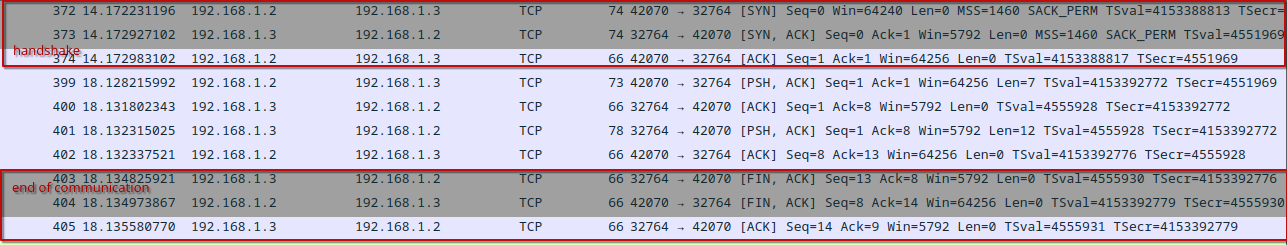
\includegraphics[width=\textwidth]{example.png}
	\caption{Capture of the exploit traffic}
\end{figure}
when analyzing the traffic we can notice the data that we sent and as the answer we get, 53 63 4d 4d ff ff ff ff 00 00 00 00 which translates to ScMM. Based on the work of \href{https://github.com/elvanderb/TCP-32764}{Eloi Vanderbken} : you can use this exploit to get remote code execution on the device. Going into some reverse engineering of the vulnerable binary.
\end{document}
